\documentclass[a4paper]{article}

\addtolength{\hoffset}{-2.25cm}
\addtolength{\textwidth}{4.5cm}
\addtolength{\voffset}{-3.25cm}
\addtolength{\textheight}{5cm}
\setlength{\parskip}{0pt}
\setlength{\parindent}{0in}

%----------------------------------------------------------------------------------------
%	PACKAGES AND OTHER DOCUMENT CONFIGURATIONS
%----------------------------------------------------------------------------------------

\usepackage{blindtext} % Package to generate dummy text
\usepackage{charter} % Use the Charter font
\usepackage[utf8]{inputenc} % Use UTF-8 encoding
\usepackage{microtype} % Slightly tweak font spacing for aesthetics
\usepackage[english]{babel} % Language hyphenation and typographical rules
\usepackage{amsthm, amsmath, amssymb} % Mathematical typesetting
\usepackage{float} % Improved interface for floating objects
\usepackage[final, colorlinks = true,
            linkcolor = black,
            citecolor = black]{hyperref} % For hyperlinks in the PDF
\usepackage{graphicx, multicol} % Enhanced support for graphics
\usepackage{xcolor} % Driver-independent color extensions
\usepackage{marvosym, wasysym} % More symbols
\usepackage{rotating} % Rotation tools
\usepackage{censor} % Facilities for controlling restricted text
\usepackage{listings} % Environment for non-formatted code, !uses style file!
\usepackage{pseudocode} % Environment for specifying algorithms in a natural way
 % Environment for f-structures, !uses style file!
\usepackage{booktabs} % Enhances quality of tables
\usepackage{tikz-qtree} % Easy tree drawing tool
 % Configuration for b-trees and b+-trees, !uses style file!
\usepackage[backend=biber,style=numeric,
            sorting=nyt]{biblatex} % Complete reimplementation of bibliographic facilities
\addbibresource{ecl.bib}
\usepackage{csquotes} % Context sensitive quotation facilities
\usepackage[yyyymmdd]{datetime} % Uses YEAR-MONTH-DAY format for dates
\renewcommand{\dateseparator}{-} % Sets dateseparator to '-'
\usepackage{fancyhdr} % Headers and footers
\pagestyle{fancy} % All pages have headers and footers
\fancyhead{}\renewcommand{\headrulewidth}{0pt} % Blank out the default header
\fancyfoot[L]{} % Custom footer text
\fancyfoot[C]{} % Custom footer text
\fancyfoot[R]{\thepage} % Custom footer text
\newcommand{\note}[1]{\marginpar{\scriptsize \textcolor{red}{#1}}} % Enables comments in red on margin
\usepackage{mathtools}
\usepackage{amsmath}
\DeclarePairedDelimiter\abs{\lvert}{\rvert}%
\usepackage{cancel}
\usepackage{minted}
\usepackage{float}
\usepackage{caption}
\usepackage{subcaption}
%-------------------------------

%----------------------------------------------------------------------------------------

%-------------------------------
%	ENVIRONMENT SECTION
%-------------------------------
\pagestyle{fancy}
\usepackage{mdframed}

\usepackage[sfdefault]{FiraSans} %% option 'sfdefault' activates Fira Sans as the default text font
\usepackage[T1]{fontenc}
\renewcommand*\oldstylenums[1]{{\firaoldstyle #1}}


% remove numbering from sections
\usepackage{titlesec}
\titleformat{\section}{\normalfont\Large\bfseries}{}{0pt}{}



%-------------------------------------------------------------------------------------------
%	CUSTOM COMMANDS
%-------------------------------
\newcommand{\gaussian}{\frac{1}{\sigma\sqrt{2\pi}}\exp\left(- \frac{(x-\mu)^2}{2\sigma^2}\right)}
\newcommand{\R}{\mathbb R}

\def\inline{\lstinline[basicstyle=\ttfamily,keywordstyle={}]}


\begin{document}


%-------------------------------
%	TITLE SECTION
%-------------------------------

\fancyhead[C]{}
\hrule \medskip % Upper rule
\begin{minipage}{0.295\textwidth}
\raggedright
\footnotesize
Francisco Javier Sáez Maldonado \hfill\\
franciscojavier.saez@estudiante.uam.es
\hfill\\
\end{minipage}
\begin{minipage}{0.4\textwidth}
\centering
\large
Face Recognition Lab Report\\
\normalsize
Deep Learning for Biometric Signal Processing\\
\end{minipage}
\begin{minipage}{0.295\textwidth}
\raggedleft
\today\hfill\\
\end{minipage}
\medskip\hrule

%-------------------------------
%	CONTENTS
%-------------------------------
\section{Task 1}

Based on the provided code, run the “FaceRecognition.m” file and complete the following points.

\subsection{Paste one image of the ATT Face Dataset and the corresponding image after using the 2D Discrete Cosine Transform (DCT)}

Firstly, I randomly changed the pre-set image to load and show. The one selected was the one shown in Figure \ref{fig:ex1a}


\begin{figure}[H]
  \centering
       \begin{subfigure}[t]{0.45\textwidth}
         \centering
         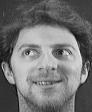
\includegraphics{Figures/Original}
         \caption{Original Image: \emph{s07/3.pgm}.}
     \end{subfigure}%
     \quad
     \begin{subfigure}[t]{0.45\textwidth}
         \centering
         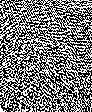
\includegraphics{Figures/Original-DCT}
         \caption{DCT applied to original image.}
     \end{subfigure}
    \caption{Examples of fingerprints.}
    \label{fig:ex1a}
\end{figure}


\subsection{Using the original configuration parameters (\inline{train = 6} images, \inline{test = 4} images, DCT \inline{coefficients = 10}), plot the resulting DET image and indicate the resulting EER.}






\subsection{Find out the configuration of the DCT coefficients that achieves the best EER results (keeping train = 6 images, test = 4 images). Justify your result, including the resulting DET image and EER value.}







\subsection{ Once selected the best configuration of the DCT coefficients (in previous point), analyze the influence of the number of training images in the system performance. Include the EER result achieved for each case (from \(train = 1\) to \(train = 7\)). Justify the results.}




\section{Task 2}
The goal of this task is to change the feature extraction module. Instead of using DCT coefficients as in Task 1, you must consider Principal Component Analysis (PCA) to extract more robust features. 
You can use the pca.m function available in Matlab. For the training phase, you should follow:
\begin{minted}{MatLab}
[coeff_PCA,MatrixTrainPCAFeats,latent] = pca(MatrixTrainFeats);
meanTrainMatrix=mean(MatrixTrainFeats);
\end{minted}
It is important to remark that the PCA function must be applied once for all training users and samples (not one PCA per user as this would provide specific \inline{coeff_PCA} parameters per user).  
For the test phase, you should follow:
\begin{quote}
For each test, subtract the meanTrainMatrix, and multiply by the \inline{coeff_PCA} transformation matrix in order to obtain the test features in the PCA domain.
\end{quote}
For more information, check Matlab Help: \url{https://es.mathworks.com/help/stats/pca.html}

\subsection{ Using the parameters train = 6 and test = 4, paste the DET curve and indicate the EER when using all the PCA components.}






\subsection{ A key aspect for the PCA is the number of components considered. Analyze and represent how the EER value changes in terms of the number of PCA components. Give your explanation about the results achieved.}


\subsection{ Indicate the optimal number of PCA components and paste the resulting DET curve together with the EER achieved. Compare the results using PCA with the DCT features considered in Task 1.}




\section{Extra Task}

The goal of this task is to improve the matching module. Instead of using a simple distance comparison, you must consider Support Vector Machines (SVM). In this case, you should train one specific SVM model per user using the training data (train = 6 images).
Features extracted using the PCA module developed in Task 2 must be considered in this Task. 
You can use the fitcsvm function available in Matlab. For the training phase, you should follow:
\begin{minted}{MatLab}
SVMModel = fitcsvm(…)
\end{minted}
For the test phase, you should follow:
\begin{minted}{MatLab}
[label,score]= predict(SVMModel,MatrixTestFeats);
\end{minted}
to obtain the scores for each user model. 
For more information, check Matlab Help:
\url{https://es.mathworks.com/help/stats/fitcsvm.html?lang=en} 
\subsection{ Using the parameters train = 6 and test = 4, paste the DET curves and indicate the EERs in the following cases: 1) regarding the KernelFunction parameter of the SVM (using all PCA components), and 2) regarding the number of PCA components considered for the feature extraction module (using the KernelFunction polynomial and starting with 3 PCA components).}




















\end{document}